%%%%%%%%%%%%%%%%%%%%%%%%%%%%%%%%%%%%%%%%%
% R Markdown: Creating Reproducible Reports
% Theme: NO \usetheme (custom footline only)
%%%%%%%%%%%%%%%%%%%%%%%%%%%%%%%%%%%%%%%%%

\documentclass[dvipsnames,hyperref={pdfpagelabels=false}]{beamer}
\usepackage{ragged2e}
\renewcommand{\raggedright}{\leftskip=0pt \rightskip=0pt plus 0cm}
\usepackage{listings}
\usepackage{lmodern}
\usepackage{fontspec}
\usepackage{xeCJK}
\setCJKmainfont{Noto Sans CJK TC}
\setCJKsansfont{Noto Sans CJK TC}
\setCJKmonofont{Noto Sans Mono CJK TC}
\usepackage[english]{babel}
\usepackage{amsmath,amssymb,amsfonts,amsthm}
\hypersetup{colorlinks=true,urlcolor=blue,citecolor=blue,pdfborder={0 0 0}}
\usepackage{tikz}
\usetikzlibrary{arrows.meta,positioning,shapes.geometric}
\usepackage{booktabs}
\usepackage{xcolor}
\usepackage{colortbl}

% R code listings style
\lstdefinestyle{rslide}{
  language=R,
  basicstyle=\footnotesize\ttfamily,
  keywordstyle=\color{NavyBlue},
  stringstyle=\color{Maroon},
  commentstyle=\color{OliveGreen},
  breaklines=true,
  frame=single,
  numbers=none,
  showstringspaces=false,
  backgroundcolor=\color{gray!6},
}
\lstset{style=rslide}

% ---- Theme block (no \usetheme) ----
\setbeamertemplate{footline}{%
  \hfill\usebeamercolor[fg]{page number in head/foot}%
  \usebeamerfont{page number in head/foot}%
  \insertframenumber\,/\,\inserttotalframenumber\hspace{1em}\vspace{2pt}%
}
\beamersetuncovermixins{\opaqueness<1>{25}}{\opaqueness<2->{15}}

\title[]{R Markdown \\ Creating Reproducible Reports}
\author{Prof.\ Tzu-Ting Yang \\ 楊子霆}
\institute{Institute of Economics, Academia Sinica \\ 中央研究院經濟研究所}
\date{\today}

\begin{document}

% ============================================================
% 1. Title frame
% ============================================================
\begin{frame}{}
  \titlepage
\end{frame}

% ============================================================
% Section divider: What Is R Markdown?
% ============================================================
\title[]{What Is R Markdown?}
\author{}\institute{}\date{}
\begin{frame}{}
  \titlepage
\end{frame}

% ============================================================
% 2. Frame: What Is R Markdown?
% ============================================================
\begin{frame}{What Is R Markdown?}
  \begin{itemize}
    \item A \texttt{.Rmd} file mixes narrative text (Markdown) + R code chunks
    \item When knitted: R runs the code, captures output \& figures
    \item \texttt{rmarkdown} converts the result into a polished \textbf{HTML} (or PDF) report
    \item Similar to Stata Markdown --- but for R, and \textbf{simpler to set up}
  \end{itemize}

  \vspace{0.8em}
  \begin{center}
    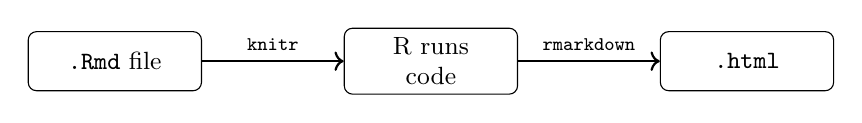
\begin{tikzpicture}[
        node distance=1.8cm,
        box/.style={rectangle, draw, rounded corners=3pt,
                    minimum width=2.2cm, minimum height=0.75cm,
                    align=center, font=\small},
        lbl/.style={font=\scriptsize, above}
      ]
      \node[box] (rmd) {\texttt{.Rmd} file};
      \node[box, right=of rmd] (rrun) {R runs\\code};
      \node[box, right=of rrun] (html) {\texttt{.html}};

      \draw[->, thick] (rmd) -- node[lbl]{\texttt{knitr}} (rrun);
      \draw[->, thick] (rrun) -- node[lbl]{\texttt{rmarkdown}} (html);
    \end{tikzpicture}
  \end{center}
\end{frame}

% ============================================================
% 3. Frame: Why Use R Markdown?
% ============================================================
\begin{frame}{Why Use R Markdown?}
  \begin{itemize}
    \item \textbf{One file, everything inside}: code + output + figures + explanation
          $\to$ single self-contained \texttt{.html}
    \item \textbf{No separate Pandoc install}: \texttt{rmarkdown} bundles Pandoc
          automatically --- simpler than Stata Markdown
    \item \textbf{Fully reproducible}: knitting always regenerates the same report
    \item \textbf{Easy to submit}: one \texttt{.html} captures your entire empirical workflow
  \end{itemize}

  \vspace{1em}
  \begin{center}
    \alert{Goal: produce one \texttt{.html} file recording all code and results}
  \end{center}
\end{frame}

% ============================================================
% Section divider: Course Templates on Dropbox
% ============================================================
\title[]{Course Templates on Dropbox}
\author{}\institute{}\date{}
\begin{frame}{}
  \titlepage
\end{frame}

% ============================================================
% 4. Frame: Course Templates on Dropbox
% ============================================================
\begin{frame}{Course Templates on Dropbox}
  \begin{center}
    \begin{tabular}{ll}
      \toprule
      \textbf{Folder} & \textbf{Contents} \\
      \midrule
      \texttt{R\_code/} & Regular \texttt{.R} scripts --- reference for R code \\
      \texttt{R\_code/R\_Markdown/} & Ready-to-knit \texttt{.Rmd} templates --- \textbf{main reference} \\
      \bottomrule
    \end{tabular}
  \end{center}

  \vspace{1em}
  Open the \texttt{.Rmd} template closest to your method and follow its structure.
\end{frame}

% ============================================================
% 5. Frame: Available .Rmd Templates
% ============================================================
\begin{frame}{Available \texttt{.Rmd} Templates}
  \begin{columns}[t]
    \column{0.48\textwidth}
    \begin{itemize}
      \item \texttt{regression.Rmd}
      \item \texttt{DID.Rmd}
      \item \texttt{Stag\_DID.Rmd}
      \item \texttt{Syn\_DID.Rmd}
      \item \texttt{fixed\_effects.Rmd}
      \item \texttt{matching.Rmd}
    \end{itemize}

    \column{0.48\textwidth}
    \begin{itemize}
      \item \texttt{RDD.Rmd}
      \item \texttt{IV.Rmd}
      \item \texttt{SSIV.Rmd}
      \item \texttt{SCM.Rmd}
      \item \texttt{ML.Rmd}
    \end{itemize}
  \end{columns}

  \vspace{1em}
  \begin{center}
    \alert{``Each template is a complete working example $\to$ knit it first,
    then adapt to your own data''}
  \end{center}
\end{frame}

% ============================================================
% Section divider: One-Time Setup
% ============================================================
\title[]{One-Time Setup}
\author{}\institute{}\date{}
\begin{frame}{}
  \titlepage
\end{frame}

% ============================================================
% 6. Frame: What You Need to Install
% ============================================================
\begin{frame}{What You Need to Install}
  \begin{center}
    \begin{tabular}{lll}
      \toprule
      \textbf{Step} & \textbf{What} & \textbf{Where} \\
      \midrule
      1 & R (base language)      & \texttt{cran.r-project.org} \\
      2 & RStudio (IDE)          & \texttt{posit.co/download/rstudio-desktop} \\
      3 & \texttt{rmarkdown} R package & Inside R Console \\
      4 & \texttt{knitr} R package     & Inside R Console \\
      \bottomrule
    \end{tabular}
  \end{center}

  \vspace{1em}
  \textit{No separate Pandoc installation needed ---
  \texttt{rmarkdown} bundles it automatically!}
\end{frame}

% ============================================================
% 7. Frame: Steps 1 & 2: Install R and RStudio [fragile]
% ============================================================
\begin{frame}[fragile]{Steps 1 \& 2: Install R and RStudio}
  \textbf{Step 1 --- Install R}:
  \begin{itemize}
    \item Go to \url{https://cran.r-project.org} $\to$ choose your OS $\to$ download
          and run installer
    \item Accept all default settings
  \end{itemize}

  \vspace{0.8em}
  \textbf{Step 2 --- Install RStudio}:
  \begin{itemize}
    \item Go to \url{https://posit.co/download/rstudio-desktop} $\to$ free Desktop version
    \item \alert{Always install R first, then RStudio}
  \end{itemize}
\end{frame}

% ============================================================
% 8. Frame: Steps 3 & 4: Install R Packages [fragile]
% ============================================================
\begin{frame}[fragile]{Steps 3 \& 4: Install R Packages}
  Run once in the RStudio Console:
  \begin{lstlisting}[style=rslide]
install.packages(c("rmarkdown", "knitr"))
  \end{lstlisting}

  \vspace{0.5em}
  Also install analysis packages for the course:
  \begin{lstlisting}[style=rslide]
install.packages(c(
  "haven",       # read Stata .dta files
  "dplyr",       # data manipulation
  "ggplot2",     # graphs
  "fixest",      # fixed effects / IV
  "estimatr",    # robust SEs
  "broom",       # tidy output
  "modelsummary" # regression tables
))
  \end{lstlisting}

  \vspace{0.3em}
  Verify: \texttt{rmarkdown::pandoc\_version()} $\to$ prints bundled Pandoc version \checkmark
\end{frame}

% ============================================================
% Section divider: Writing Your .Rmd File
% ============================================================
\title[]{Writing Your \texttt{.Rmd} File}
\author{}\institute{}\date{}
\begin{frame}{}
  \titlepage
\end{frame}

% ============================================================
% 9. Frame: Structure of a .Rmd File [fragile]
% ============================================================
\begin{frame}[fragile]{Structure of a \texttt{.Rmd} File}
  \begin{enumerate}
    \item \textbf{YAML header} (between \texttt{-{}-{}-} lines): title, author, output options
    \item \textbf{Markdown text}: narrative, headings with \texttt{\#} / \texttt{\#\#}
    \item \textbf{R code chunks}: fenced with \texttt{```\{r chunkname\}} \ldots{} \texttt{```}
  \end{enumerate}

  \vspace{0.5em}
  \begin{lstlisting}[language={},backgroundcolor=\color{gray!6}]
---
title: "My Report"
author: "Your Name"
output:
  html_document:
    toc: true
    toc_float: true
    theme: flatly
---
  \end{lstlisting}
\end{frame}

% ============================================================
% 10. Frame: The Setup Chunk [fragile]
% ============================================================
\begin{frame}[fragile]{The Setup Chunk}
  Placed immediately after the YAML header. Sets global options and file paths.

  \begin{lstlisting}[style=rslide]
```{r setup, include=FALSE}
knitr::opts_chunk$set(echo=TRUE, warning=FALSE, message=FALSE)
rm(list = ls())

username <- Sys.info()[["user"]]
if (username == "alice") {
  rawdata <- "C:/Users/alice/Desktop/data"
} else if (username == "bob") {
  rawdata <- "/Users/bob/Documents/data"
}
```
  \end{lstlisting}

  \vspace{0.3em}
  \begin{itemize}
    \item \texttt{include=FALSE}: chunk runs but nothing appears in the HTML
    \item Use \texttt{Sys.info()[["user"]]} to find your username (run in Console)
  \end{itemize}
\end{frame}

% ============================================================
% 11. Frame: Chunk Options [fragile]
% ============================================================
\begin{frame}[fragile]{Chunk Options}
  \small
  \begin{center}
    \begin{tabular}{lll}
      \toprule
      \textbf{Option} & \textbf{Default} & \textbf{Effect} \\
      \midrule
      \texttt{echo}    & \texttt{TRUE} & Show R code in report \\
      \texttt{eval}    & \texttt{TRUE} & Run the code \\
      \texttt{include} & \texttt{TRUE} & Include any output at all \\
      \texttt{warning} & \texttt{TRUE} & Show R warnings \\
      \texttt{message} & \texttt{TRUE} & Show messages from \texttt{library()} \\
      \bottomrule
    \end{tabular}
  \end{center}

  \vspace{0.5em}
  Always use \texttt{eval=FALSE} for install chunks:
  \begin{lstlisting}[style=rslide]
```{r packages, eval=FALSE}
install.packages(c("haven", "ggplot2", "fixest"))
```
  \end{lstlisting}

  \texttt{eval=FALSE}: code is displayed but NOT run during knitting ---
  always use for \texttt{install.packages()}
\end{frame}

% ============================================================
% 12. Frame: Portable Path Setup [fragile]
% ============================================================
\begin{frame}[fragile]{Portable Path Setup}
  \textbf{Problem}: hard-coded paths break on other computers.

  \textbf{Solution}: use \texttt{Sys.info()[["user"]]}:

  \begin{lstlisting}[style=rslide]
username <- Sys.info()[["user"]]
if (username == "alice") {
  rawdata <- "C:/Users/alice/Desktop/data"
} else if (username == "bob") {
  rawdata <- "/Users/bob/Documents/data"
}
  \end{lstlisting}

  \vspace{0.3em}
  Then use throughout:
  \begin{lstlisting}[style=rslide]
df <- read_dta(file.path(rawdata, "mydata.dta"))
  \end{lstlisting}

  \vspace{0.3em}
  Find your username: run \texttt{Sys.info()[["user"]]} in the R Console.
\end{frame}

% ============================================================
% Section divider: Compile to HTML
% ============================================================
\title[]{Compile to HTML}
\author{}\institute{}\date{}
\begin{frame}{}
  \titlepage
\end{frame}

% ============================================================
% 13. Frame: Compile: Two Methods [fragile]
% ============================================================
\begin{frame}[fragile]{Compile: Two Methods}
  \textbf{Method A --- Knit button} (recommended for beginners):
  \begin{itemize}
    \item Click the blue \textbf{Knit} button at the top of the RStudio editor
    \item RStudio saves \texttt{file.html} and opens it in the Viewer automatically
  \end{itemize}

  \vspace{0.8em}
  \textbf{Method B --- R Console}:
  \begin{lstlisting}[style=rslide]
rmarkdown::render("myreport.Rmd")
  \end{lstlisting}

  \vspace{0.5em}
  \begin{center}
    \alert{Output: \texttt{myreport.html} in the same folder as your \texttt{.Rmd}
    --- open in any browser!}
  \end{center}
\end{frame}

% ============================================================
% 14. Frame: HTML Is Self-Contained by Default [fragile]
% ============================================================
\begin{frame}[fragile]{HTML Is Self-Contained by Default}
  \textbf{R Markdown HTML} (default behavior):
  \begin{itemize}
    \item All figures embedded inline $\to$ single portable file
    \item No \texttt{bundle} option needed (unlike Stata Markdown)
    \item Just submit \texttt{yourfile.html} --- nothing else required
  \end{itemize}

  \vspace{0.8em}
  \textbf{Optional: control output with \texttt{render()}}:
  \begin{lstlisting}[style=rslide]
rmarkdown::render("myreport.Rmd",
  output_file = "myreport.html",
  output_dir  = "C:/output/")
  \end{lstlisting}
\end{frame}

% ============================================================
% Section divider: Troubleshooting
% ============================================================
\title[]{Troubleshooting}
\author{}\institute{}\date{}
\begin{frame}{}
  \titlepage
\end{frame}

% ============================================================
% 15. Frame: Common Errors
% ============================================================
\begin{frame}{Common Errors}
  \small
  \begin{center}
    \begin{tabular}{ll}
      \toprule
      \textbf{Problem} & \textbf{Fix} \\
      \midrule
      \texttt{could not find function "feols"} & Add \texttt{library(fixest)} at top of \texttt{.Rmd} \\
      \texttt{there is no package called 'X'}  & Run \texttt{install.packages("X")} in Console \\
      \texttt{cannot open file: No such file}  & Check path setup chunk and \texttt{Sys.info()[["user"]]} \\
      Figures not showing                      & Remove \texttt{include=FALSE} from that chunk \\
      Knit fails at \texttt{install.packages()} & Use \texttt{eval=FALSE} on install chunks \\
      Code output missing                      & Check \texttt{echo=FALSE} is not blocking that chunk \\
      \bottomrule
    \end{tabular}
  \end{center}
\end{frame}

% ============================================================
% Section divider: Summary
% ============================================================
\title[]{Summary}
\author{}\institute{}\date{}
\begin{frame}{}
  \titlepage
\end{frame}

% ============================================================
% 16. Frame: Setup Checklist
% ============================================================
\begin{frame}{Setup Checklist}
  \begin{enumerate}
    \item $\square$ Install R from \url{cran.r-project.org}
    \item $\square$ Install RStudio from \url{posit.co/download/rstudio-desktop}
    \item $\square$ \texttt{install.packages(c("rmarkdown","knitr"))} in Console
    \item $\square$ Install analysis packages: \texttt{haven, dplyr, ggplot2, fixest, \ldots}
    \item $\square$ Verify: \texttt{rmarkdown::pandoc\_version()} prints a version
    \item $\square$ Write \texttt{.Rmd}: YAML header + setup chunk + \texttt{```\{r\}} blocks
    \item $\square$ Set paths with \texttt{Sys.info()[["user"]]} in the setup chunk
    \item $\square$ Use \texttt{eval=FALSE} on \texttt{install.packages()} chunks
    \item $\square$ Click \textbf{Knit} (or \texttt{rmarkdown::render("file.Rmd")})
    \item $\square$ Open \texttt{file.html} in browser $\checkmark$
  \end{enumerate}
\end{frame}

\end{document}
